%%%%%%%%%%%%%%%%%%%%%%%%%%%%%%%%%%%%%%%%%%%%%%%%%%%%%%%%%%%%%%%%%%%%%%%%%%%%%%%%%%%%%%%%%%%%%%
\begin{toepassing}
	\label{wolkenkrabber}
Een wolkenkrabber kan vereenvoudigd worden als een balk met grondvlakzijden van 50m en een hoogte van 300m. De weerstandscoëfficiënt van een vierkante sectie is 2.2. Volgens metingen is de gemiddelde windsnelheid afhankelijk van de hoogte volgens $v = C z^{0.40}$.

Indien 3 dimensionale effecten aan de top van de wolkenkrabber verwaarloosd kunnen worden, bepaal dan de totale kracht en het krachtverdeling functie van de hoogte die de wind uitoefent indien op een hoogte van 10m de windsnelheid 5m/s bedraagt.
\end{toepassing}
\begin{antwoord}{\ref{wolkenkrabber}}
	$f = \unit{N/m}$, $F = \unit{N}$
\end{antwoord}
%%%%%%%%%%%%%%%%%%%%%%%%%%%%%%%%%%%%%%%%%%%%%%%%%%%%%%%%%%%%%%%%%%%%%%%%%%%%%%%%%%%%%%%%%%%%%%
\begin{toepassing}[*]
	\label{airbus}
Een volgeladen Airbus A380 weegt 650ton, het totale vleugeloppervlak is 845\unit{m^2}. De vleugels zijn opgebouwd uit NACA SC(2) 0610 profielen met een lift en weerstands karakteristiek zoals hieronder weergegeven. De romp vereenvoudigen we als een cilinder met 8m diameter en een weerstandscoëfficiënt van 1.2. De weerstand van de staart en de ophanging van de motoren worden verwaarloosd. De gewenste kruissnelheid is 900km/u. De dichtheid van lucht op de kruishoogte is ongeveer 0.35\unit{kg/m^3}.
		
Bepaal de aanvalshoek van de vleugels nodig voor horizontale vlucht aan kruissnelheid en de stuwkracht die de motoren moeten leveren in deze omstandigheden.

	\centering
	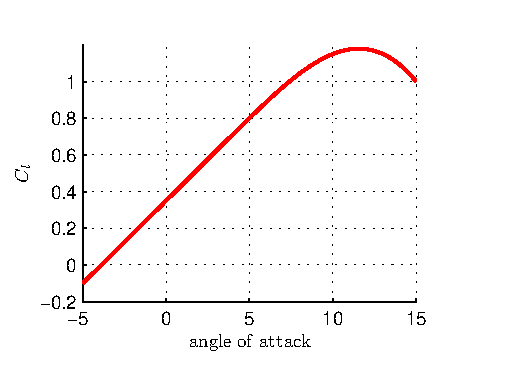
\includegraphics[width=0.48\textwidth]{fig/uitwendige_stroming/NACA_SC(2)_0610_Cl.pdf}
	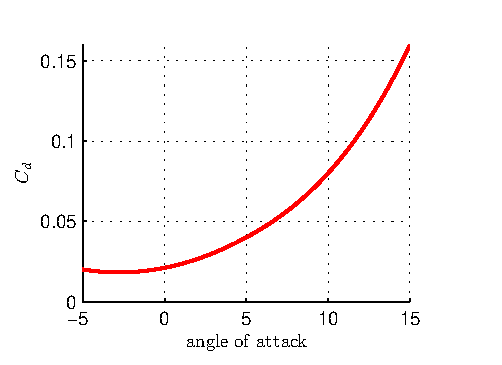
\includegraphics[width=0.48\textwidth]{fig/uitwendige_stroming/NACA_SC(2)_0610_Cd.pdf}
\end{toepassing}
\begin{antwoord}{\ref{airbus}}
	$\alpha \approx 4\deg$, $F \approx 983\unit{kN}$
\end{antwoord}
%%%%%%%%%%%%%%%%%%%%%%%%%%%%%%%%%%%%%%%%%%%%%%%%%%%%%%%%%%%%%%%%%%%%%%%%%%%%%%%%%%%%%%%%%%%%%%


\section*{Antwoorden}
	\begin{multicols}{2}
		\includecollection{antwoorden}
	\end{multicols}